% ============================================================
% 初升高衔接讲义 — 一元二次方程与二次函数
% 编译命令：xelatex -interaction=nonstopmode 衔接1_一元二次方程与二次函数.tex
% ============================================================
\documentclass[12pt, a4paper]{ctexart}
\usepackage[margin=2.2cm]{geometry}
\usepackage{amsmath, amssymb}
\usepackage{enumitem}
\usepackage{tcolorbox}
\usepackage{booktabs}
\usepackage{array}
\usepackage{fancyhdr}
\usepackage{xcolor}
\usepackage{tikz}
\usepackage{hyperref}
\usepackage{graphicx}
\usepackage{multirow}
\usepackage{pgfplots}
\pgfplotsset{compat=1.18}

% 颜色定义
\definecolor{mainblue}{RGB}{41, 98, 168}
\definecolor{lightblue}{RGB}{230, 240, 255}
\definecolor{tipgreen}{RGB}{34, 139, 87}
\definecolor{lightgreen}{RGB}{235, 250, 240}
\definecolor{warnred}{RGB}{200, 50, 50}
\definecolor{lightred}{RGB}{255, 240, 240}
\definecolor{examorange}{RGB}{210, 120, 20}
\definecolor{lightorange}{RGB}{255, 248, 235}
\definecolor{apppurple}{RGB}{120, 60, 170}
\definecolor{lightpurple}{RGB}{245, 238, 255}

% 页眉页脚
\pagestyle{fancy}
\fancyhf{}
\fancyhead[L]{\small\textcolor{mainblue}{\textbf{初升高衔接 \(\cdot\) 一元二次方程与二次函数}}}
\fancyhead[R]{\small\textcolor{mainblue}{衔接讲义}}
\fancyfoot[C]{\small —\ \thepage\ —}
\renewcommand{\headrulewidth}{0.6pt}
\renewcommand{\headrule}{\hbox to\headwidth{\color{mainblue}\leaders\hrule height \headrulewidth\hfill}}
\renewcommand{\footrulewidth}{0pt}

% tcolorbox 样式
\newtcolorbox{knowledgebox}[1][]{%
  colback=lightblue, colframe=mainblue,
  fonttitle=\bfseries\large, title=#1,
  arc=3mm, boxrule=0.8pt,
  left=8pt, right=8pt, top=6pt, bottom=6pt
}

\newtcolorbox{tipbox}[1][]{%
  colback=lightgreen, colframe=tipgreen,
  fonttitle=\bfseries, title=#1,
  arc=2mm, boxrule=0.6pt,
  left=6pt, right=6pt, top=4pt, bottom=4pt
}

\newtcolorbox{warnbox}[1][]{%
  colback=lightred, colframe=warnred,
  fonttitle=\bfseries, title=#1,
  arc=2mm, boxrule=0.6pt,
  left=6pt, right=6pt, top=4pt, bottom=4pt
}

\newtcolorbox{examplebox}[1][]{%
  colback=lightorange, colframe=examorange,
  fonttitle=\bfseries, title=#1,
  arc=3mm, boxrule=0.8pt,
  left=8pt, right=8pt, top=6pt, bottom=6pt
}

\newtcolorbox{appbox}[1][]{%
  colback=lightpurple, colframe=apppurple,
  fonttitle=\bfseries, title=#1,
  arc=3mm, boxrule=0.8pt,
  left=8pt, right=8pt, top=6pt, bottom=6pt
}

\setCJKmainfont{Hiragino Sans GB}
\setCJKsansfont{Heiti SC}

\begin{document}

% ============ 标题页 ============
\begin{center}
{\Huge\bfseries\textcolor{mainblue}{一元二次方程与二次函数}}\\[12pt]
{\Large\textcolor{gray}{初升高衔接讲义}}\\[8pt]
\rule{0.6\textwidth}{1pt}\\[8pt]
{\normalsize 适用：准高一新生 \quad|\quad 课时：2--3课时}
\end{center}
\vspace{10pt}

% ============ 第一部分：知识点讲解 ============
\section*{\textcolor{mainblue}{一、知识点讲解}}

% ---- 1.1 一元二次方程的定义 ----
\subsection*{1.1\quad 一元二次方程的定义}

\begin{knowledgebox}[什么是"一元二次方程"？]
形如
\[
ax^2 + bx + c = 0 \quad (a \neq 0)
\]
的方程叫做\textbf{一元二次方程}。

其中：
\begin{itemize}[leftmargin=2em]
  \item $a$ 叫做\textbf{二次项系数}（$a \neq 0$，这是关键条件！）
  \item $b$ 叫做\textbf{一次项系数}
  \item $c$ 叫做\textbf{常数项}
\end{itemize}
"一元"表示只有\textbf{一个}未知数；"二次"表示未知数的\textbf{最高次数}为 2。
\end{knowledgebox}

\begin{warnbox}[易错提醒]
判断一个方程是否为一元二次方程，必须先化为标准形式 $ax^2+bx+c=0$，再看：
\begin{enumerate}[leftmargin=2em]
  \item 只含一个未知数；
  \item 最高次数是 2；
  \item 二次项系数 $a \neq 0$。
\end{enumerate}
例如：$(m-1)x^2 + 3x - 5 = 0$ 是一元二次方程的条件是 $m \neq 1$。
\end{warnbox}

% ---- 1.2 四种解法 ----
\subsection*{1.2\quad 一元二次方程的四种解法}

\begin{knowledgebox}[方法一：直接开平方法]
\textbf{适用情况：} 方程可以写成 $(\text{含未知数的式子})^2 = \text{常数}$ 的形式。

\textbf{基本原理：} 若 $x^2 = p$（$p \geq 0$），则 $x = \pm\sqrt{p}$。

\textbf{例：} 解方程 $(x - 3)^2 = 16$

\textbf{解题步骤：}
\begin{enumerate}[leftmargin=2em]
  \item 两边同时开平方（注意正负两个根）：
  \[
  x - 3 = \pm\sqrt{16} = \pm 4
  \]
  \item 分别解两个一元一次方程：
  \[
  x - 3 = 4 \implies x = 7
  \]
  \[
  x - 3 = -4 \implies x = -1
  \]
  \item 所以方程的解为 $x_1 = 7,\; x_2 = -1$。
\end{enumerate}
\end{knowledgebox}

\begin{knowledgebox}[方法二：配方法]
\textbf{适用情况：} 通用方法，适用于所有一元二次方程。

\textbf{核心思想：} 通过配方，把方程变成 $(\text{含未知数的式子})^2 = \text{常数}$ 的形式，再用开平方法求解。

\textbf{配方公式（要牢记）：}
\[
ax^2 + bx + c = a\!\left(x + \frac{b}{2a}\right)^{\!2} - \frac{b^2 - 4ac}{4a}
\]

\textbf{例：} 解方程 $x^2 + 6x + 5 = 0$

\textbf{详细步骤：}
\begin{enumerate}[leftmargin=2em]
  \item 把常数项移到等号右边：
  \[
  x^2 + 6x = -5
  \]
  \item 等号两边同时加上"一次项系数一半的平方"。一次项系数是 6，一半是 3，平方是 9：
  \[
  x^2 + 6x + 9 = -5 + 9
  \]
  \item 左边写成完全平方的形式，右边计算：
  \[
  (x + 3)^2 = 4
  \]
  \item 两边开平方：
  \[
  x + 3 = \pm 2
  \]
  \item 分别求解：
  \[
  x + 3 = 2 \implies x = -1
  \]
  \[
  x + 3 = -2 \implies x = -5
  \]
  \item 所以 $x_1 = -1,\; x_2 = -5$。
\end{enumerate}
\end{knowledgebox}

\begin{warnbox}[配方法的关键步骤]
配方时，\textbf{两边都要加}，不能只加一边！加的数是"一次项系数一半的平方"，即 $\left(\dfrac{b}{2}\right)^2$。\vspace{4pt}

\textbf{验算习惯：} 把求出的 $x$ 值代回原方程，检验等号是否成立。
\end{warnbox}

\begin{knowledgebox}[方法三：公式法]
\textbf{适用情况：} 通用方法，适用于所有一元二次方程。

\textbf{求根公式：} 对于 $ax^2 + bx + c = 0$（$a \neq 0$），当 $\Delta = b^2 - 4ac \geq 0$ 时：
\[
\boxed{x = \frac{-b \pm \sqrt{b^2 - 4ac}}{2a}}
\]

\textbf{例：} 解方程 $2x^2 - 5x - 3 = 0$

\textbf{详细步骤：}
\begin{enumerate}[leftmargin=2em]
  \item 确定 $a, b, c$ 的值：$a = 2,\; b = -5,\; c = -3$。
  \item 计算判别式：
  \[
  \Delta = b^2 - 4ac = (-5)^2 - 4 \times 2 \times (-3) = 25 + 24 = 49
  \]
  \item 因为 $\Delta = 49 > 0$，方程有两个不相等的实数根。
  \item 代入求根公式：
  \[
  x = \frac{-(-5) \pm \sqrt{49}}{2 \times 2} = \frac{5 \pm 7}{4}
  \]
  \item 分别计算：
  \[
  x_1 = \frac{5 + 7}{4} = \frac{12}{4} = 3, \qquad x_2 = \frac{5 - 7}{4} = \frac{-2}{4} = -\frac{1}{2}
  \]
  \item 所以 $x_1 = 3,\; x_2 = -\dfrac{1}{2}$。
\end{enumerate}
\end{knowledgebox}

\begin{knowledgebox}[方法四：因式分解法]
\textbf{适用情况：} 当方程左边容易因式分解时使用，是\textbf{最快}的方法。

\textbf{核心思想：} 如果 $A \times B = 0$，那么 $A = 0$ 或 $B = 0$。

\textbf{例：} 解方程 $x^2 - 5x + 6 = 0$

\textbf{详细步骤：}
\begin{enumerate}[leftmargin=2em]
  \item 尝试把左边因式分解。找两个数，使它们的积为 $+6$，和为 $-5$。
  \item 这两个数是 $-2$ 和 $-3$（因为 $(-2) \times (-3) = 6$，$(-2) + (-3) = -5$）。
  \item 因式分解：
  \[
  x^2 - 5x + 6 = (x - 2)(x - 3) = 0
  \]
  \item 令每个因式等于零：
  \[
  x - 2 = 0 \implies x_1 = 2
  \]
  \[
  x - 3 = 0 \implies x_2 = 3
  \]
  \item 所以 $x_1 = 2,\; x_2 = 3$。
\end{enumerate}
\end{knowledgebox}

\begin{tipbox}[四种方法的选择策略]
\begin{enumerate}[leftmargin=2em]
  \item \textbf{先看能否因式分解}——能的话最快（十字相乘法、提公因式法等）。
  \item \textbf{再看是否适合直接开平方}——方程为 $(x+m)^2 = n$ 形式时。
  \item \textbf{配方法}是通用方法，也是推导求根公式的基础，要重点掌握。
  \item \textbf{公式法}是万能方法，记住公式即可，但计算量可能较大。
\end{enumerate}
\end{tipbox}

% ---- 1.3 判别式 ----
\subsection*{1.3\quad 判别式 $\Delta$ 的意义}

\begin{knowledgebox}[判别式]
对于一元二次方程 $ax^2 + bx + c = 0$（$a \neq 0$），定义
\[
\boxed{\Delta = b^2 - 4ac}
\]

\begin{center}
\renewcommand{\arraystretch}{1.5}
\begin{tabular}{|c|c|c|}
\hline
\textbf{$\Delta$ 的值} & \textbf{根的情况} & \textbf{图象与 $x$ 轴} \\
\hline
$\Delta > 0$ & 两个\textbf{不相等}的实数根 & 两个交点 \\
\hline
$\Delta = 0$ & 两个\textbf{相等}的实数根（重根） & 一个交点（相切） \\
\hline
$\Delta < 0$ & \textbf{没有}实数根 & 无交点 \\
\hline
\end{tabular}
\end{center}
\end{knowledgebox}

\begin{warnbox}[易错提醒]
\begin{itemize}[leftmargin=2em]
  \item $\Delta < 0$ 时，方程没有\textbf{实数}根，但有\textbf{虚数}根（高中阶段一般不作要求）。
  \item 使用求根公式前，\textbf{必须先算} $\Delta$，判断根的情况。
  \item $\Delta$ 的计算不要忘记 $a$ 前面的符号：$b^2 - 4ac$，不是 $b^2 + 4ac$。
\end{itemize}
\end{warnbox}

% ---- 1.4 韦达定理 ----
\subsection*{1.4\quad 韦达定理（根与系数的关系）}

\begin{knowledgebox}[韦达定理]
设 $x_1, x_2$ 是一元二次方程 $ax^2 + bx + c = 0$（$a \neq 0$，$\Delta \geq 0$）的两个根，则：
\[
\boxed{x_1 + x_2 = -\frac{b}{a}}, \qquad \boxed{x_1 \cdot x_2 = \frac{c}{a}}
\]

\textbf{记忆口诀：} 两根之和等于"一次项系数除以二次项系数"的\textbf{相反数}；两根之积等于"常数项除以二次项系数"。
\end{knowledgebox}

\begin{tipbox}[韦达定理的常见应用]
\begin{enumerate}[leftmargin=2em]
  \item \textbf{已知两根，求原方程：} 若两根为 $x_1, x_2$，则方程为
  \[
  x^2 - (x_1 + x_2)x + x_1 x_2 = 0
  \]
  \item \textbf{求关于两根的对称式：} 如 $x_1^2 + x_2^2 = (x_1+x_2)^2 - 2x_1 x_2$，
  \[
  \frac{1}{x_1} + \frac{1}{x_2} = \frac{x_1 + x_2}{x_1 x_2}, \quad
  (x_1 - x_2)^2 = (x_1+x_2)^2 - 4x_1 x_2
  \]
  \item \textbf{判断根的正负：} 利用 $x_1 + x_2$ 和 $x_1 x_2$ 的符号判断。
\end{enumerate}
\end{tipbox}

% ---- 1.5 二次函数三种表达式 ----
\subsection*{1.5\quad 二次函数的三种表达式}

\begin{knowledgebox}[三种表达式对比]
\begin{center}
\renewcommand{\arraystretch}{1.8}
\begin{tabular}{|c|c|c|}
\hline
\textbf{名称} & \textbf{形式} & \textbf{特点} \\
\hline
一般式 & $y = ax^2 + bx + c$ & 直接看出 $c$（$y$ 轴截距） \\
\hline
顶点式 & $y = a(x - h)^2 + k$ & 直接看出顶点 $(h, k)$ \\
\hline
交点式 & $y = a(x - x_1)(x - x_2)$ & 直接看出与 $x$ 轴交点 \\
\hline
\end{tabular}
\end{center}

\textbf{三种形式之间的转换：}
\begin{itemize}[leftmargin=2em]
  \item 一般式 $\to$ 顶点式：用\textbf{配方法}。
  \item 一般式 $\to$ 交点式：先解方程 $ax^2+bx+c=0$ 得两根 $x_1, x_2$，再写成 $a(x-x_1)(x-x_2)$。
  \item 顶点式 $\to$ 一般式：展开即可。
\end{itemize}
\end{knowledgebox}

% ---- 1.6 二次函数图象与性质 ----
\subsection*{1.6\quad 二次函数图象与性质}

\begin{knowledgebox}[二次函数 $y = ax^2 + bx + c$ 的图象与性质]
二次函数的图象是一条\textbf{抛物线}。

\textbf{关键性质：}
\begin{enumerate}[leftmargin=2em]
  \item \textbf{开口方向：}
  \begin{itemize}
    \item $a > 0$：开口\textbf{向上}（像碗口朝上）。
    \item $a < 0$：开口\textbf{向下}（像碗口朝下）。
  \end{itemize}
  \item \textbf{对称轴：}
  \[
  x = -\frac{b}{2a}
  \]
  \item \textbf{顶点坐标：}
  \[
  \left(-\frac{b}{2a},\; \frac{4ac - b^2}{4a}\right)
  \]
  用顶点式 $y = a(x-h)^2 + k$ 时，顶点为 $(h, k)$。
  \item \textbf{最值：}
  \begin{itemize}
    \item $a > 0$ 时，顶点处取\textbf{最小值} $y_{\min} = \dfrac{4ac - b^2}{4a}$。
    \item $a < 0$ 时，顶点处取\textbf{最大值} $y_{\max} = \dfrac{4ac - b^2}{4a}$。
  \end{itemize}
  \item \textbf{增减性：}（以对称轴 $x = -\dfrac{b}{2a}$ 为分界）
  \begin{itemize}
    \item $a > 0$ 时：在对称轴左侧 $y$ 随 $x$ 增大而减小；右侧 $y$ 随 $x$ 增大而增大。
    \item $a < 0$ 时：在对称轴左侧 $y$ 随 $x$ 增大而增大；右侧 $y$ 随 $x$ 增大而减小。
  \end{itemize}
\end{enumerate}
\end{knowledgebox}

\begin{warnbox}[记忆技巧]
"左同右异"——在对称轴的\textbf{左边}，$a$ 和 $x$ 的变化方向\textbf{相同}（$a>0$时$y$增大，$a<0$时$y$减小）；在\textbf{右边}则\textbf{相反}。\vspace{4pt}

更简单的记忆：$a > 0$ 开口向上，先减后增；$a < 0$ 开口向下，先增后减。
\end{warnbox}

% ---- 1.7 a/b/c符号与图象关系 ----
\subsection*{1.7\quad $a$, $b$, $c$ 的符号与图象的关系}

\begin{knowledgebox}[看图判断 $a$, $b$, $c$ 的符号]
\begin{center}
\renewcommand{\arraystretch}{1.6}
\begin{tabular}{|c|p{10cm}|}
\hline
\textbf{符号} & \textbf{判断方法} \\
\hline
$a$ 的符号 & 看\textbf{开口方向}：开口向上则 $a > 0$，开口向下则 $a < 0$。\\
\hline
$c$ 的符号 & 看图象与\textbf{$y$ 轴交点}的位置：交于 $y$ 轴正半轴则 $c > 0$，交于负半轴则 $c < 0$，过原点则 $c = 0$。\\
\hline
$b$ 的符号 & 看\textbf{对称轴}位置，结合 $a$ 的符号判断：对称轴 $x = -\dfrac{b}{2a}$ 在 $y$ 轴\textbf{右侧}（即 $-\dfrac{b}{2a} > 0$），若 $a > 0$ 则 $b < 0$；在\textbf{左侧}则 $b > 0$。\vspace{2pt}\\
& \textbf{简记：}"左同右异"——对称轴在 $y$ 轴左边时 $a, b$ 同号；右边时异号。\\
\hline
$\Delta$ 的符号 & 看图象与\textbf{$x$ 轴}交点个数：有 2 个交点则 $\Delta > 0$，1 个则 $\Delta = 0$，无交点则 $\Delta < 0$。\\
\hline
\end{tabular}
\end{center}
\end{knowledgebox}

% ---- 1.8 二次函数与方程的关系 ----
\subsection*{1.8\quad 二次函数与一元二次方程的关系}

\begin{knowledgebox}[核心联系]
二次函数 $y = ax^2 + bx + c$ 的图象与 $x$ 轴的交点，就是方程 $ax^2 + bx + c = 0$ 的\textbf{实数根}。

\begin{center}
\renewcommand{\arraystretch}{1.5}
\begin{tabular}{|c|c|c|}
\hline
\textbf{图象与 $x$ 轴} & \textbf{$\Delta$ 的值} & \textbf{方程的根} \\
\hline
两个交点 $(x_1, 0)$, $(x_2, 0)$ & $\Delta > 0$ & 两个不相等的实根 \\
\hline
一个交点 $(x_0, 0)$ & $\Delta = 0$ & 两个相等的实根（重根） \\
\hline
没有交点 & $\Delta < 0$ & 无实根 \\
\hline
\end{tabular}
\end{center}

\textbf{换句话说：} 求方程 $ax^2 + bx + c = 0$ 的根，就是在求抛物线 $y = ax^2 + bx + c$ 与 $x$ 轴交点的横坐标。
\end{knowledgebox}

% ---- 1.9 二次不等式 ----
\subsection*{1.9\quad 一元二次不等式（高中预习）}

\begin{knowledgebox}[用图象法解一元二次不等式]
这是高中数学的重要内容，初中只需初步了解。\vspace{6pt}

\textbf{方法步骤：}
\begin{enumerate}[leftmargin=2em]
  \item 把不等式化为标准形式 $ax^2 + bx + c > 0$（或 $< 0$，$\geq 0$，$\leq 0$）。
  \item 解对应的方程 $ax^2 + bx + c = 0$，求出两根 $x_1, x_2$（设 $x_1 < x_2$）。
  \item 画出抛物线 $y = ax^2 + bx + c$ 的草图。
  \item 根据不等号方向和开口方向，找出 $x$ 的范围。
\end{enumerate}

\textbf{口诀（$a > 0$，两根 $x_1 < x_2$ 时）：}
\begin{center}
\renewcommand{\arraystretch}{1.5}
\begin{tabular}{|c|c|}
\hline
\textbf{不等式} & \textbf{解集} \\
\hline
$ax^2 + bx + c > 0$ & $x < x_1$ 或 $x > x_2$（"大于取两边"）\\
\hline
$ax^2 + bx + c < 0$ & $x_1 < x < x_2$（"小于取中间"）\\
\hline
\end{tabular}
\end{center}

若 $a < 0$，先两边除以 $a$（注意不等号变号！），转化为 $a > 0$ 的情况。
\end{knowledgebox}

\begin{warnbox}[特别注意]
\begin{itemize}[leftmargin=2em]
  \item 解二次不等式时，\textbf{一定要画草图辅助理解}，不要死记硬背。
  \item 若 $\Delta < 0$（方程无实根），则 $a > 0$ 时 $ax^2+bx+c > 0$ 的解集为\textbf{全体实数} $\mathbb{R}$。
  \item 端点是否取等号要看" $>$ "还是" $\geq$ "。
\end{itemize}
\end{warnbox}


% ============ 第二部分：例题精讲 ============
\section*{\textcolor{examorange}{二、例题精讲}}

% 例题1：因式分解法
\begin{examplebox}[【例题 1】因式分解法解方程]
用因式分解法解方程：$x^2 - 7x + 12 = 0$。
\end{examplebox}

\textbf{解：}
\begin{enumerate}[leftmargin=2em]
  \item 观察方程左边 $x^2 - 7x + 12$，需要找两个数，使它们的：
  \begin{itemize}
    \item 积 $= 12$（常数项）
    \item 和 $= -7$（一次项系数）
  \end{itemize}
  \item 这两个数是 $-3$ 和 $-4$（因为 $(-3) \times (-4) = 12$，$(-3) + (-4) = -7$）。
  \item 因式分解：
  \[
  x^2 - 7x + 12 = (x - 3)(x - 4) = 0
  \]
  \item 令每个因式等于零：
  \[
  x - 3 = 0 \implies x_1 = 3
  \]
  \[
  x - 4 = 0 \implies x_2 = 4
  \]
  \item \textbf{答：} $x_1 = 3,\; x_2 = 4$。
\end{enumerate}

% 例题2：配方法
\begin{examplebox}[【例题 2】配方法解方程]
用配方法解方程：$x^2 - 4x - 1 = 0$。
\end{examplebox}

\textbf{解：}
\begin{enumerate}[leftmargin=2em]
  \item 移项，把常数项移到右边：
  \[
  x^2 - 4x = 1
  \]
  \item 配方：一次项系数为 $-4$，一半为 $-2$，平方为 $4$。两边同时加 $4$：
  \[
  x^2 - 4x + 4 = 1 + 4
  \]
  \item 左边写成完全平方：
  \[
  (x - 2)^2 = 5
  \]
  \item 两边开平方：
  \[
  x - 2 = \pm\sqrt{5}
  \]
  \item 求解：
  \[
  x_1 = 2 + \sqrt{5}, \qquad x_2 = 2 - \sqrt{5}
  \]
  \item \textbf{答：} $x_1 = 2 + \sqrt{5},\; x_2 = 2 - \sqrt{5}$。
\end{enumerate}

% 例题3：公式法
\begin{examplebox}[【例题 3】公式法解方程]
用公式法解方程：$3x^2 + 2x - 2 = 0$。
\end{examplebox}

\textbf{解：}
\begin{enumerate}[leftmargin=2em]
  \item 确定 $a = 3,\; b = 2,\; c = -2$。
  \item 计算判别式：
  \[
  \Delta = b^2 - 4ac = 2^2 - 4 \times 3 \times (-2) = 4 + 24 = 28 > 0
  \]
  所以方程有两个不相等的实数根。
  \item 代入求根公式：
  \[
  x = \frac{-b \pm \sqrt{\Delta}}{2a} = \frac{-2 \pm \sqrt{28}}{2 \times 3} = \frac{-2 \pm 2\sqrt{7}}{6}
  \]
  \item 化简：
  \[
  x = \frac{-1 \pm \sqrt{7}}{3}
  \]
  \item 所以：
  \[
  x_1 = \frac{-1 + \sqrt{7}}{3}, \qquad x_2 = \frac{-1 - \sqrt{7}}{3}
  \]
  \item \textbf{答：} $x_1 = \dfrac{-1 + \sqrt{7}}{3},\; x_2 = \dfrac{-1 - \sqrt{7}}{3}$。
\end{enumerate}

% 例题4：判别式应用
\begin{examplebox}[【例题 4】判别式的应用]
已知关于 $x$ 的方程 $x^2 + 2x + m = 0$ 有两个不相等的实数根，求 $m$ 的取值范围。
\end{examplebox}

\textbf{解：}
\begin{enumerate}[leftmargin=2em]
  \item 方程有两个不相等的实数根，则判别式 $\Delta > 0$。
  \item 这里 $a = 1,\; b = 2,\; c = m$。
  \item 计算判别式：
  \[
  \Delta = b^2 - 4ac = 2^2 - 4 \times 1 \times m = 4 - 4m
  \]
  \item 令 $\Delta > 0$：
  \[
  4 - 4m > 0
  \]
  \[
  -4m > -4
  \]
  \[
  m < 1
  \]
  \item \textbf{答：} 当 $m < 1$ 时，方程有两个不相等的实数根。
\end{enumerate}

\begin{warnbox}[易错提醒]
解不等式 $4 - 4m > 0$ 时，两边除以 $-4$，不等号要\textbf{变向}！这是常见错误。
\end{warnbox}

% 例题5：韦达定理
\begin{examplebox}[【例题 5】韦达定理应用]
已知方程 $x^2 - 5x + 3 = 0$ 的两个根为 $x_1, x_2$，不解方程，求 $x_1^2 + x_2^2$ 的值。
\end{examplebox}

\textbf{解：}
\begin{enumerate}[leftmargin=2em]
  \item 由韦达定理（$a = 1,\; b = -5,\; c = 3$）：
  \[
  x_1 + x_2 = -\frac{b}{a} = -\frac{-5}{1} = 5
  \]
  \[
  x_1 \cdot x_2 = \frac{c}{a} = \frac{3}{1} = 3
  \]
  \item 利用恒等式转化：
  \[
  x_1^2 + x_2^2 = (x_1 + x_2)^2 - 2x_1 x_2
  \]
  \item 代入数值：
  \[
  x_1^2 + x_2^2 = 5^2 - 2 \times 3 = 25 - 6 = 19
  \]
  \item \textbf{答：} $x_1^2 + x_2^2 = 19$。
\end{enumerate}

\begin{tipbox}[方法总结]
遇到"不解方程，求关于两根的式子"，优先考虑：
\begin{itemize}[leftmargin=2em]
  \item $x_1^2 + x_2^2 = (x_1+x_2)^2 - 2x_1x_2$
  \item $(x_1 - x_2)^2 = (x_1+x_2)^2 - 4x_1x_2$
  \item $\dfrac{1}{x_1} + \dfrac{1}{x_2} = \dfrac{x_1+x_2}{x_1 x_2}$
\end{itemize}
这些恒等式要熟记。
\end{tipbox}

% 例题6：配方求顶点
\begin{examplebox}[【例题 6】配方求二次函数顶点]
将二次函数 $y = 2x^2 - 8x + 10$ 化为顶点式，并写出顶点坐标和对称轴。
\end{examplebox}

\textbf{解：}
\begin{enumerate}[leftmargin=2em]
  \item 提取二次项系数（只从含 $x$ 的项中提取）：
  \[
  y = 2(x^2 - 4x) + 10
  \]
  \item 对括号内配方：一次项系数为 $-4$，一半为 $-2$，平方为 $4$。
  \[
  y = 2(x^2 - 4x + 4 - 4) + 10
  \]
  注意：括号内加了 $4$，为了不改变式子的值，要减去 $4$。
  \item 整理：
  \[
  y = 2(x^2 - 4x + 4) - 2 \times 4 + 10 = 2(x - 2)^2 - 8 + 10
  \]
  \item 化简得到顶点式：
  \[
  y = 2(x - 2)^2 + 2
  \]
  \item \textbf{答：} 顶点式为 $y = 2(x-2)^2 + 2$，顶点坐标为 $(2,\; 2)$，对称轴为 $x = 2$。
\end{enumerate}

\begin{warnbox}[配方的关键]
提出系数 $2$ 后，括号内加的数必须再乘以 $2$ 才能"还回去"。
即 $y = 2\big[(x-2)^2 - 4\big] + 10 = 2(x-2)^2 - 8 + 10$。
\end{warnbox}

% 例题7：看图判断abc符号
\begin{examplebox}[【例题 7】根据图象判断 $a$, $b$, $c$ 的符号]
如图所示为二次函数 $y = ax^2 + bx + c$ 的图象，请判断 $a$, $b$, $c$, $b^2 - 4ac$ 的正负。

\begin{center}
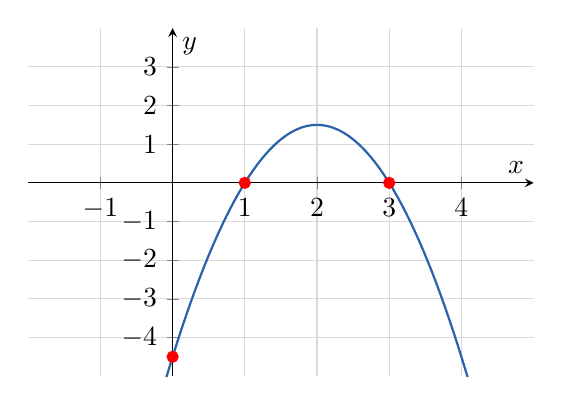
\begin{tikzpicture}
\begin{axis}[
  axis lines=middle,
  xlabel=$x$, ylabel=$y$,
  xmin=-2, xmax=5, ymin=-5, ymax=4,
  xtick={-1,0,1,2,3,4},
  ytick={-4,-3,-2,-1,0,1,2,3},
  grid=major,
  grid style={gray!30},
  width=8cm, height=6cm,
]
\addplot[domain=-1.5:4.5, samples=100, thick, mainblue]
  {-1.5*(x-1)*(x-3) + 0};
\addplot[only marks, mark=*, mark size=2pt, red] coordinates {(1,0) (3,0)};
\addplot[only marks, mark=*, mark size=2pt, red] coordinates {(0,-4.5)};
\end{axis}
\end{tikzpicture}
\end{center}
\end{examplebox}

\textbf{解：} 逐个分析：
\begin{enumerate}[leftmargin=2em]
  \item \textbf{判断 $a$ 的符号：} 抛物线开口\textbf{向下}，所以 $a < 0$。
  \item \textbf{判断 $c$ 的符号：} 图象与 $y$ 轴交于\textbf{负半轴}（$y$ 截距为负），所以 $c < 0$。
  \item \textbf{判断 $b$ 的符号：}
  \begin{itemize}
    \item 对称轴在 $y$ 轴\textbf{右侧}（本图中对称轴约为 $x = 2$）。
    \item 对称轴 $x = -\dfrac{b}{2a} > 0$。
    \item 因为 $a < 0$，所以 $-\dfrac{b}{2a} > 0 \implies \dfrac{b}{2a} < 0$。
    \item 分母 $2a < 0$，要使分式 $< 0$，分子 $b$ 必须 $> 0$。
    \item 所以 $b > 0$。
  \end{itemize}
  \item \textbf{判断 $\Delta = b^2 - 4ac$ 的符号：} 图象与 $x$ 轴有\textbf{两个交点}，所以 $\Delta > 0$。
\end{enumerate}

\textbf{答：} $a < 0$，$b > 0$，$c < 0$，$b^2 - 4ac > 0$。

% 例题8：二次函数与方程综合
\begin{examplebox}[【例题 8】二次函数与方程综合]
已知二次函数 $y = x^2 - 2x - 3$。
\begin{enumerate}[label=(\arabic*)]
  \item 求图象与 $x$ 轴的交点坐标；
  \item 求顶点坐标；
  \item 当 $x$ 取何值时，$y > 0$？
\end{enumerate}
\end{examplebox}

\textbf{解：}

（1）求与 $x$ 轴交点，令 $y = 0$：
\[
x^2 - 2x - 3 = 0
\]
因式分解：$(x - 3)(x + 1) = 0$

$x_1 = 3,\; x_2 = -1$

所以与 $x$ 轴交点为 $(-1,\; 0)$ 和 $(3,\; 0)$。

（2）配方求顶点：
\[
y = x^2 - 2x - 3 = (x^2 - 2x + 1) - 1 - 3 = (x - 1)^2 - 4
\]
顶点为 $(1,\; -4)$。

（3）由 $y > 0$ 得：
\[
(x - 1)^2 - 4 > 0 \implies (x - 1)^2 > 4
\]
\[
|x - 1| > 2
\]
\[
x - 1 > 2 \text{ 或 } x - 1 < -2
\]
\[
x > 3 \text{ 或 } x < -1
\]

\textbf{答：}（1）与 $x$ 轴交点为 $(-1,0)$ 和 $(3,0)$；（2）顶点为 $(1,-4)$；（3）$x > 3$ 或 $x < -1$ 时 $y > 0$。

\begin{tipbox}[方法总结]
" $y > 0$ "就是"图象在 $x$ 轴\textbf{上方}的部分"。画出草图后，很容易看出 $x$ 的范围。也可以用前面的口诀："大于取两边"，即 $x < -1$ 或 $x > 3$。
\end{tipbox}

% 例题9：含参二次方程
\begin{examplebox}[【例题 9】含参问题]
已知关于 $x$ 的方程 $(m-1)x^2 + 2mx + (m+3) = 0$ 有一个根为 $0$，求 $m$ 的值及另一个根。
\end{examplebox}

\textbf{解：}
\begin{enumerate}[leftmargin=2em]
  \item 因为 $x = 0$ 是方程的根，将 $x = 0$ 代入方程：
  \[
  (m - 1) \times 0^2 + 2m \times 0 + (m + 3) = 0
  \]
  \[
  m + 3 = 0
  \]
  \[
  m = -3
  \]
  \item 将 $m = -3$ 代回原方程：
  \[
  (-3 - 1)x^2 + 2 \times (-3) \times x + (-3 + 3) = 0
  \]
  \[
  -4x^2 - 6x = 0
  \]
  \item 提取公因式：
  \[
  -2x(2x + 3) = 0
  \]
  \item 解得：$x = 0$ 或 $2x + 3 = 0 \implies x = -\dfrac{3}{2}$。
  \item 验证 $m - 1 = -4 \neq 0$，确实是一元二次方程。
  \item \textbf{答：} $m = -3$，另一个根为 $x = -\dfrac{3}{2}$。
\end{enumerate}

% 例题10：二次不等式
\begin{examplebox}[【例题 10】解一元二次不等式]
解不等式：$x^2 - 5x + 6 < 0$。
\end{examplebox}

\textbf{解：}
\begin{enumerate}[leftmargin=2em]
  \item 先解对应的方程 $x^2 - 5x + 6 = 0$：
  \[
  (x - 2)(x - 3) = 0 \implies x_1 = 2,\; x_2 = 3
  \]
  \item 画抛物线 $y = x^2 - 5x + 6$ 的草图：
  \begin{itemize}
    \item $a = 1 > 0$，开口向上。
    \item 与 $x$ 轴交于 $x = 2$ 和 $x = 3$。
  \end{itemize}
  \begin{center}
  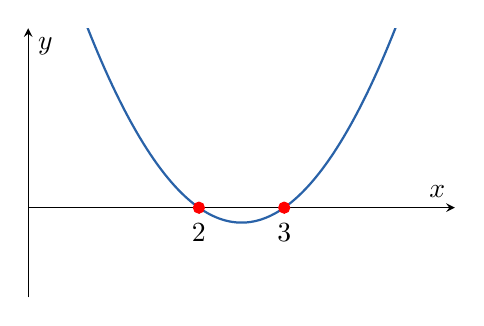
\begin{tikzpicture}
  \begin{axis}[
    axis lines=middle,
    xlabel=$x$, ylabel=$y$,
    xmin=0, xmax=5, ymin=-1.5, ymax=3,
    xtick={2,3},
    xticklabels={$2$,$3$},
    ytick=\empty,
    width=7cm, height=5cm,
  ]
  \addplot[domain=0.5:4.5, samples=100, thick, mainblue]
    {(x-2)*(x-3)};
  \addplot[only marks, mark=*, mark size=2pt, red] coordinates {(2,0) (3,0)};
  \end{axis}
  \end{tikzpicture}
  \end{center}
  \item $y < 0$ 对应图象在 $x$ 轴下方的部分，即 $2 < x < 3$。
  \item \textbf{答：} 不等式的解集为 $2 < x < 3$（即 $x \in (2,\; 3)$）。
\end{enumerate}


% ============ 第三部分：应用题 ============
\section*{\textcolor{apppurple}{三、应用题}}

\begin{appbox}[【应用 1】利润最大化问题]
某商店以每件 $30$ 元的成本进了一批商品。根据市场调查，当售价为每件 $x$ 元时（$x \geq 30$），每天可卖出 $(100 - 2x)$ 件。问：售价定为多少元时，每天的利润最大？最大利润是多少？
\end{appbox}

\textbf{解：}
\begin{enumerate}[leftmargin=2em]
  \item 设每件售价为 $x$ 元。
  \item 每件利润为 $(x - 30)$ 元。
  \item 每天销售量为 $(100 - 2x)$ 件。
  \item 每天的总利润 $W$ 为：
  \[
  W = (x - 30)(100 - 2x)
  \]
  \item 展开整理：
  \[
  W = 100x - 2x^2 - 3000 + 60x = -2x^2 + 160x - 3000
  \]
  \item 这是一个 $a = -2 < 0$ 的二次函数，开口向下，有最大值。
  \item 配方：
  \[
  W = -2(x^2 - 80x) - 3000
  \]
  \[
  W = -2(x^2 - 80x + 1600 - 1600) - 3000
  \]
  \[
  W = -2(x - 40)^2 + 3200 - 3000
  \]
  \[
  W = -2(x - 40)^2 + 200
  \]
  \item 当 $x = 40$ 时，$W$ 取最大值 $200$ 元。
  \item 验证合理性：$x = 40 \geq 30$（合理），此时销售量 $= 100 - 2 \times 40 = 20 > 0$（合理）。
  \item \textbf{答：} 售价定为每件 $40$ 元时，每天利润最大，最大利润为 $200$ 元。
\end{enumerate}

\begin{appbox}[【应用 2】面积最值问题]
用一段长为 $24$ 米的篱笆围成一个一面靠墙的矩形花园（墙的长度足够），设垂直于墙的一边长为 $x$ 米。
\begin{enumerate}[label=(\arabic*)]
  \item 用 $x$ 表示花园的面积 $S$；
  \item 当 $x$ 为多少米时，花园面积最大？最大面积是多少？
\end{enumerate}
\end{appbox}

\textbf{解：}

（1）
\begin{itemize}[leftmargin=2em]
  \item 设垂直于墙的边长为 $x$ 米。
  \item 因为一面靠墙，所以篱笆只围三面。平行于墙的边长为 $(24 - 2x)$ 米。
  \item 注意 $x > 0$ 且 $24 - 2x > 0$，即 $0 < x < 12$。
  \item 面积：
  \[
  S = x(24 - 2x) = 24x - 2x^2
  \]
\end{itemize}

（2）
\begin{itemize}[leftmargin=2em]
  \item 配方：
  \[
  S = -2(x^2 - 12x) = -2(x^2 - 12x + 36 - 36) = -2(x - 6)^2 + 72
  \]
  \item 因为 $a = -2 < 0$，开口向下，当 $x = 6$ 时，$S$ 取最大值 $72$。
  \item 验证：$x = 6$ 满足 $0 < x < 12$，此时平行于墙的边长 $= 24 - 12 = 12$ 米，合理。
  \item \textbf{答：} 当 $x = 6$ 米时，花园面积最大，最大面积为 $72$ 平方米。
\end{itemize}

\begin{appbox}[【应用 3】抛物线形拱桥问题]
一座抛物线形拱桥，桥拱的跨度为 $20$ 米，拱高为 $4$ 米。在桥拱上距离左端 $5$ 米处有一根竖直的支撑柱。求这根支撑柱的高度。
\end{appbox}

\textbf{解：}
\begin{enumerate}[leftmargin=2em]
  \item 建立坐标系：以桥拱的最低点（即桥拱最高点下方的端点）为原点，水平方向为 $x$ 轴，竖直方向为 $y$ 轴。
  \begin{itemize}
    \item 更好的做法：以桥拱最高点为坐标原点，这样抛物线方程更简单。
    \item 设桥拱最高点为原点 $O$，水平向右为 $x$ 轴正方向，竖直向上为 $y$ 轴正方向。
    \item 则抛物线开口向下，顶点为 $(0, 0)$。
  \end{itemize}
  \item 由题意，桥拱跨度 $20$ 米，拱高 $4$ 米，则抛物线过 $(10,\; -4)$ 和 $(-10,\; -4)$。
  \item 设抛物线方程为 $y = ax^2$（顶点在原点，对称轴为 $y$ 轴）。
  \item 代入 $(10, -4)$：
  \[
  -4 = a \times 10^2 = 100a \implies a = -\frac{1}{25}
  \]
  \item 抛物线方程为：
  \[
  y = -\frac{1}{25}x^2
  \]
  \item "距离左端 $5$ 米处"，左端对应 $x = -10$，所以该点的 $x$ 坐标为 $-10 + 5 = -5$。
  \item 代入 $x = -5$：
  \[
  y = -\frac{1}{25} \times (-5)^2 = -\frac{25}{25} = -1
  \]
  \item 支撑柱的高度为该点到桥面的距离。$y = -1$ 表示在最高点下方 $1$ 米处。支撑柱从桥面向上延伸到拱桥的底部（桥面处），所以高度为拱高减去此处距最高点的距离：
  \[
  \text{支撑柱高度} = \text{拱高} - |y| = 4 - 1 = 3 \text{ 米}
  \]
  \item \textbf{答：} 支撑柱的高度为 $3$ 米。
\end{enumerate}


% ============ 第四部分：课堂练习 ============
\section*{\textcolor{tipgreen}{四、课堂练习}}

\begin{enumerate}[leftmargin=2em]
  \item 用直接开平方法解方程：$(2x - 1)^2 = 9$。

  \item 用配方法解方程：$x^2 + 4x - 1 = 0$。

  \item 用公式法解方程：$2x^2 + 3x - 2 = 0$。

  \item 用因式分解法解方程：$3x^2 - 12x = 0$。

  \item 已知方程 $x^2 - 3x + m = 0$ 有两个相等的实数根，求 $m$ 的值。

  \item 已知方程 $x^2 + 4x - 5 = 0$ 的两根为 $x_1, x_2$，不解方程，求 $\dfrac{1}{x_1} + \dfrac{1}{x_2}$ 的值。

  \item 将二次函数 $y = -x^2 + 6x - 5$ 化为顶点式，并写出顶点坐标。

  \item 解不等式：$x^2 - 4x + 3 > 0$。
\end{enumerate}

\vspace{20pt}

% ---- 参考答案 ----
\begin{knowledgebox}[参考答案]

\textbf{第 1 题：}
\[
(2x - 1)^2 = 9 \implies 2x - 1 = \pm 3
\]
\[
2x - 1 = 3 \implies x = 2; \qquad 2x - 1 = -3 \implies x = -1
\]
答：$x_1 = 2,\; x_2 = -1$。

\vspace{8pt}
\textbf{第 2 题：}
\[
x^2 + 4x = 1
\]
\[
x^2 + 4x + 4 = 1 + 4 = 5
\]
\[
(x + 2)^2 = 5
\]
\[
x + 2 = \pm\sqrt{5}
\]
答：$x_1 = -2 + \sqrt{5},\; x_2 = -2 - \sqrt{5}$。

\vspace{8pt}
\textbf{第 3 题：}
$a = 2,\; b = 3,\; c = -2$。
\[
\Delta = 9 - 4 \times 2 \times (-2) = 9 + 16 = 25
\]
\[
x = \frac{-3 \pm 5}{4}
\]
答：$x_1 = \dfrac{1}{2},\; x_2 = -2$。

\vspace{8pt}
\textbf{第 4 题：}
\[
3x^2 - 12x = 0 \implies 3x(x - 4) = 0
\]
答：$x_1 = 0,\; x_2 = 4$。

\vspace{8pt}
\textbf{第 5 题：}
两个相等的实数根 $\implies \Delta = 0$。
\[
\Delta = (-3)^2 - 4 \times 1 \times m = 9 - 4m = 0 \implies m = \frac{9}{4}
\]
答：$m = \dfrac{9}{4}$。

\vspace{8pt}
\textbf{第 6 题：}
由韦达定理：$x_1 + x_2 = -4,\; x_1 x_2 = -5$。
\[
\frac{1}{x_1} + \frac{1}{x_2} = \frac{x_1 + x_2}{x_1 x_2} = \frac{-4}{-5} = \frac{4}{5}
\]
答：$\dfrac{4}{5}$。

\vspace{8pt}
\textbf{第 7 题：}
\[
y = -(x^2 - 6x) - 5 = -(x^2 - 6x + 9 - 9) - 5 = -(x - 3)^2 + 9 - 5 = -(x - 3)^2 + 4
\]
答：顶点式 $y = -(x - 3)^2 + 4$，顶点坐标为 $(3,\; 4)$。

\vspace{8pt}
\textbf{第 8 题：}
解 $x^2 - 4x + 3 = 0$：$(x-1)(x-3)=0$，$x_1 = 1,\; x_2 = 3$。

$a = 1 > 0$，开口向上，"大于取两边"。

答：$x < 1$ 或 $x > 3$。

\end{knowledgebox}

\vfill
\begin{center}
\small\textcolor{gray}{本讲义仅供教学参考，例题可根据学生水平调整难度。}
\end{center}

\end{document}
